\documentclass[10pt,a4paper]{article}
\usepackage[utf8]{inputenc}
\usepackage{amsmath}
\usepackage{amsfonts}
\usepackage{amssymb}
\usepackage{graphicx}
\begin{document}
\section*{MobileClient Look.}
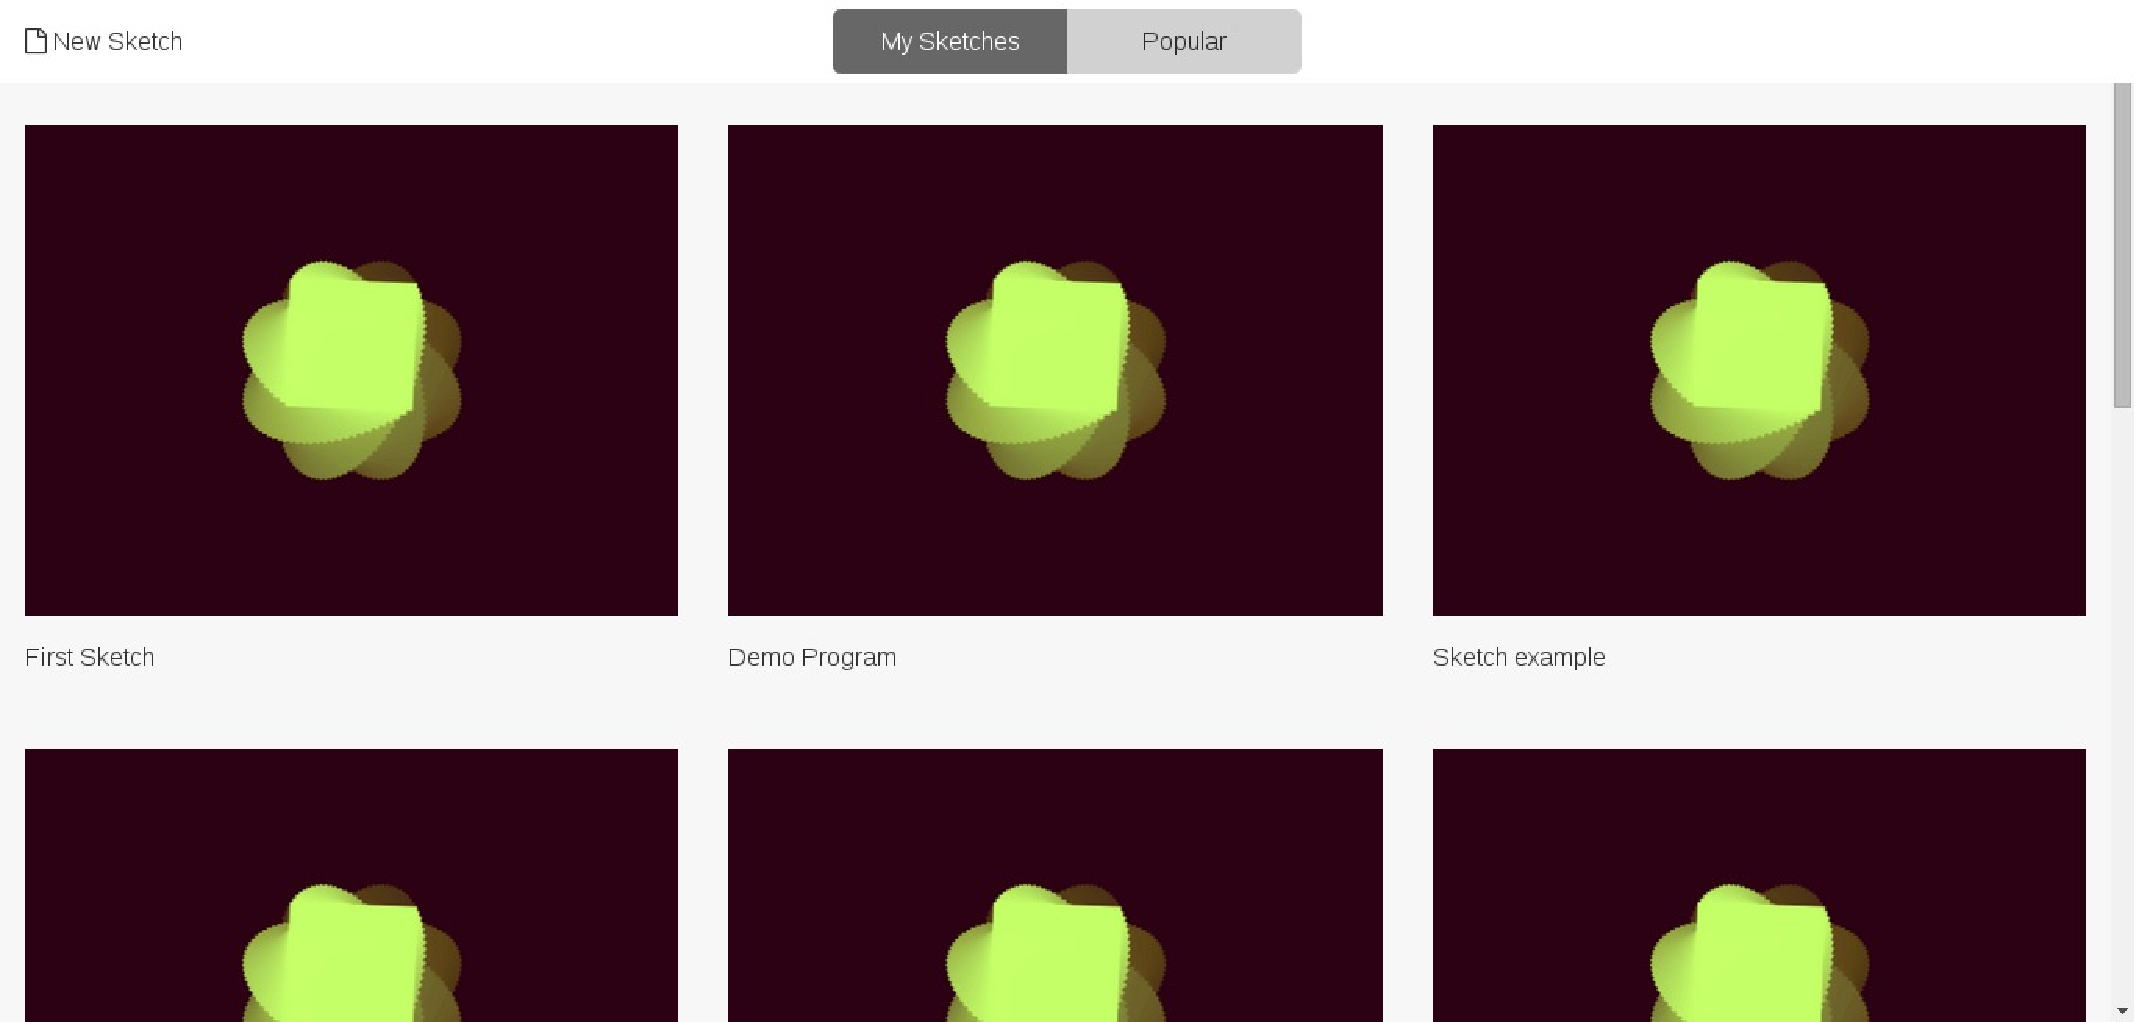
\includegraphics[width=\textwidth,keepaspectratio]{browser.pdf}
\hfill\\
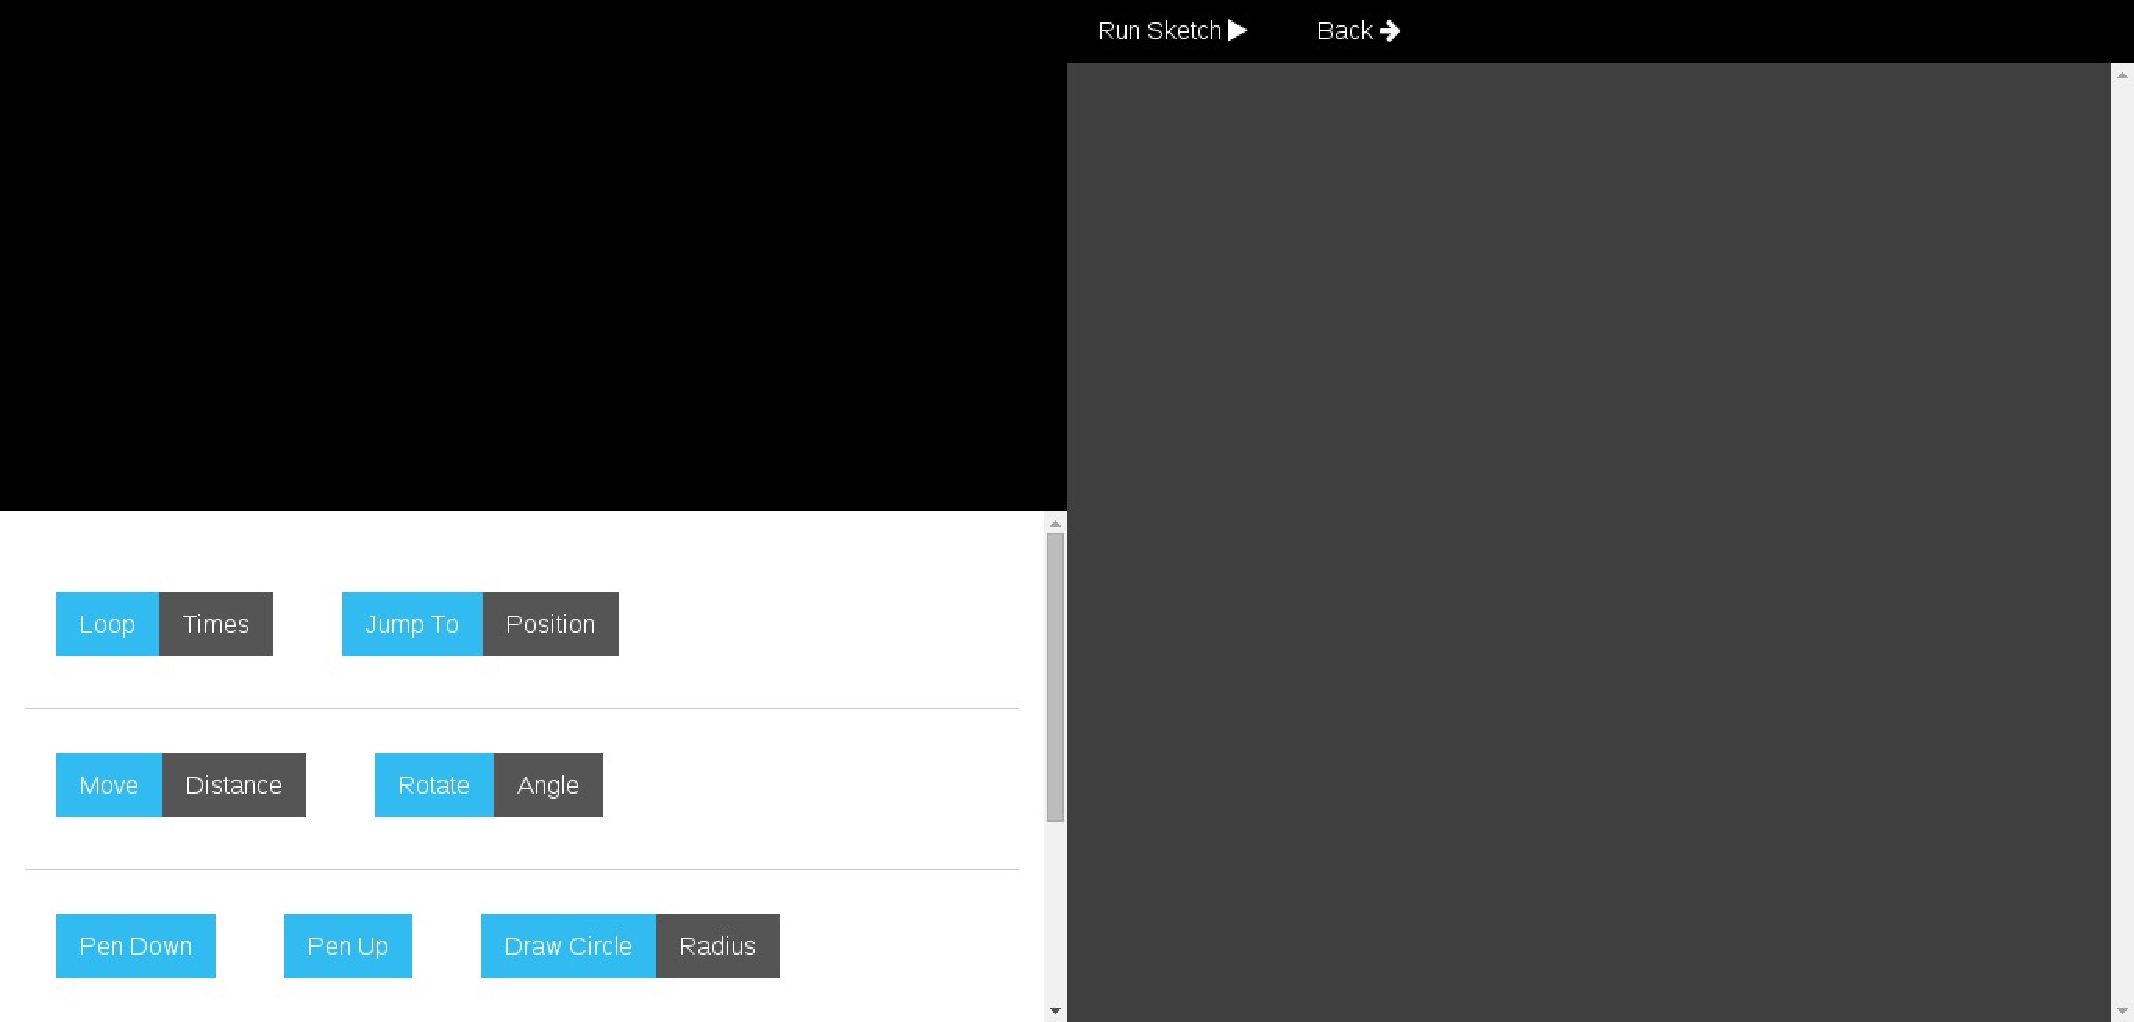
\includegraphics[width=\textwidth,keepaspectratio]{editor.pdf}
\hfill\\
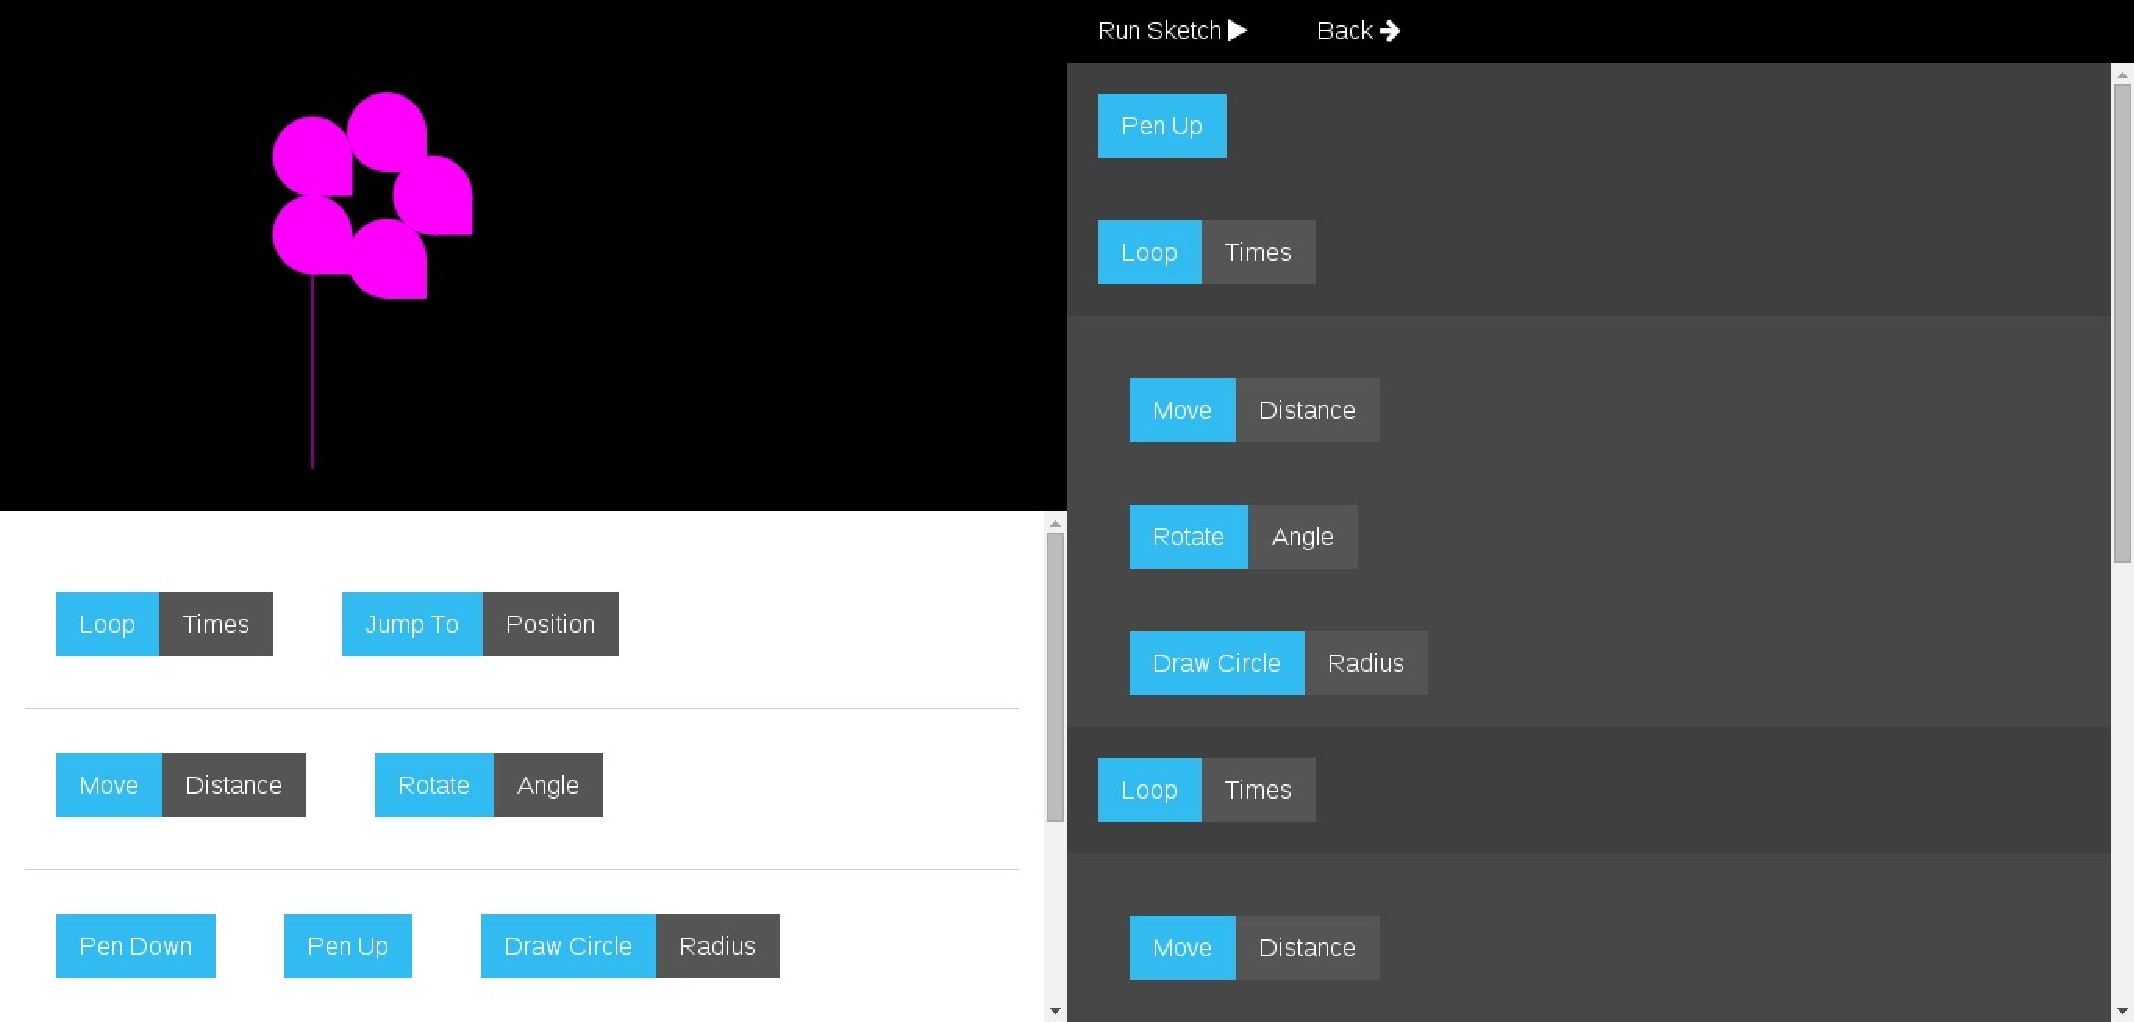
\includegraphics[width=\textwidth,keepaspectratio]{editor_with_contents.pdf}

\newpage
\section*{System Architecture.}
\begin{itemize}
\item Hosted on heroku.
\item Data teir is nodejs.
\item postgres as data teir.
\item preview images stored on s3
\item otherstuff stored in database.(postgre).
\end{itemize}
\newpage
\section*{Issues.}

\subsection*{Scalability.}
	By using stateless protocols we don't have to store anything serves side this means that very few resources are 		         	needed to process requests.
\subsection*{Security.}
	prepared statements in postgres to avoid sql injection.
	escaping on the client side to avoid xss.(encoding)
	We have identified the need to address the issue of authentication of devices to prevent unauthorised       	   of user data.
\subsubsection*{issues}
-Potential issues with binary blob.
-	
\subsection*{Reliability.}
	heroku- unlikly for hardware to fail.
	We have tested 
\subsection*{Privacy.}
\newpage
\section*{Testing.}




\end{document}